\documentclass[journal]{IEEEtran}
% Every number, table and figure in this file was generated from the per-seed logs by
% https://github.com/Abraheem13/tierfed and is written here as plain text.
\usepackage[utf8]{inputenc}
\usepackage[T1]{fontenc}
\usepackage{amsmath,amssymb,amsthm}
\usepackage{booktabs}
\usepackage{graphicx}
\usepackage{xcolor}
\usepackage{etoolbox}
\usepackage{multirow}
\usepackage{url}
\usepackage{tikz}
\usetikzlibrary{arrows.meta,positioning,fit,calc,shapes.geometric,backgrounds}
\usepackage[hidelinks]{hyperref}
\hypersetup{pdftitle={When Does Per-Tier Synchronisation Pay? A Closed-Form Test and a Traffic Side Channel in Communication-Budgeted Federated Learning}, pdfauthor={Abraheem Rashid, Mehwish Mahmood}}
\usepackage{cite}

% ---------------------------------------------------------------------------
% ---------------------------------------------------------------------------
\newsavebox\tabbox
\newcommand{\fit}[1]{\sbox\tabbox{#1}\ifdim\wd\tabbox>\linewidth\resizebox{\linewidth}{!}{\usebox\tabbox}\else\usebox\tabbox\fi}
\newcommand{\fig}[2]{\includegraphics[width=#2]{figures/#1.pdf}}

\newtheorem{proposition}{Proposition}
\newcommand{\tierfed}{TierFed}
\newcommand{\Gh}{\hat\Gamma}

% flowchart styles (Figs. 1-3)
\definecolor{srv}{RGB}{255,255,255}
\definecolor{lnk}{RGB}{255,255,255}
\definecolor{ste}{RGB}{255,255,255}
\definecolor{stg}{RGB}{255,255,255}
\tikzset{
  proc/.style={draw=black, rounded corners=1.5pt, align=center, font=\scriptsize, inner sep=3pt, minimum height=6mm, fill=stg, line width=0.5pt},
  srvbox/.style={proc, fill=srv}, lnkbox/.style={proc, fill=lnk}, stebox/.style={proc, fill=ste},
  dec/.style={draw=black, diamond, aspect=3.6, align=center, font=\scriptsize, inner sep=1.5pt, fill=white, line width=0.5pt},
  term/.style={draw=black, rounded corners=3mm, align=center, font=\scriptsize, inner sep=3pt, minimum height=5.5mm, fill=white, line width=0.5pt},
  grp/.style={draw=black, dashed, rounded corners=3pt, inner sep=5pt},
  hdr/.style={font=\scriptsize\bfseries, anchor=south},
  lab/.style={font=\scriptsize, fill=white, inner sep=1.2pt},
  arr/.style={-{Latex[length=1.8mm,width=1.4mm]}, line width=0.6pt},
  meas/.style={-{Latex[length=1.8mm,width=1.4mm]}, line width=0.6pt, dashed},
}

\raggedbottom   % leftover space at the foot of a column, not between paragraphs
\begin{document}
\bstctlcite{IEEEexample:BSTcontrol}

\title{When Does Per-Tier Synchronisation Pay? A Closed-Form Test and a Traffic Side Channel in Communication-Budgeted Federated Learning}

\author{Abraheem~Rashid and Mehwish~Mahmood
\thanks{A.~Rashid is with the Department of Computer Science, Brunel University London, Uxbridge UB8~3PH, U.K. (e-mail: 2546393@brunel.ac.uk).}
\thanks{M.~Mahmood is with Queen's University Belfast, Belfast, U.K.}
\thanks{Corresponding author: Abraheem Rashid.}}

\markboth{IEEE Transactions on Machine Learning in Communications and Networking}{Rashid and Mahmood: When Does Per-Tier Synchronisation Pay?}

\maketitle

\begin{abstract}
Federated learning over constrained links must fit a byte quota, and under client-level differential privacy (DP) every synchronisation is also a release. This article asks when synchronising parts of a model at different rates pays. The relaxed quota-constrained programme of a blockwise local-SGD surrogate has a closed form, and a H\"older bound $\Psi$, measurable at the end of warm-up, limits how much any per-tier schedule can reduce that surrogate below a uniform period. The bound is tested with \tierfed{}, which sets per-tier intervals from measured dispersion, keeps the classifier head private and staggers tiers to cap single-round payload. On a 20-site readmission benchmark $\Psi$ is 0.1\%, \tierfed{} reduces to the uniform period, and every federated method except AdaComm is within 0.0032 AUROC of full-rate FedPer, \tierfed{} sending 65.3 of FedPer's 217.8~MB. On a ResNet $\Psi$ is 71.4\% and the tiers split as predicted, yet no reading of the runs shows a relevant gain over the best uniform period at matched bytes, so the surrogate gain did not become an accuracy gain. Staggered phases cut the rounds that miss a transfer window from 0.30 to 0.08 at the cost of more radio wake-ups. Under client-level DP at 20 sites every releasing schedule ends below local training, and an adaptive scheduler's traffic reveals a site with shifted labels to a passive observer even when that site never skips an upload. A consistency check recomputes every planned release and uncompressed upload from the stated rules, and one command regenerates every number from the released logs.
\end{abstract}


\begin{IEEEkeywords}
Federated learning, communication-efficient learning, local SGD, multi-rate aggregation, network resource allocation, differential privacy, traffic analysis, clinical prediction.
\end{IEEEkeywords}

\section{Introduction}
\label{sec:intro}

\IEEEPARstart{F}{ederated} learning allows several institutions to train one predictive model without exchanging records~\cite{mcmahan2017,kairouz2021}. In cross-silo healthcare the participants are a handful of sites, each behind its own firewall on a link that its network team controls~\cite{rieke2020,dayan2021}. The learning job is one tenant on an uplink with a fixed capacity and a scheduled transfer window; whether the link is an institutional WAN, a cellular edge slice or a satellite backhaul, the operator asks how many bytes the job pushes per window, and whether they fit~\cite{lim2020,chen2021joint}.

A server coordinates $N$ sites over $R$ rounds and in each round requests some, all or none of the shared parameters. It must keep the mean fraction of the shared model transmitted per round within a quota $\rho$, keep the personalised accuracy non-inferior to full-rate personalisation and, where client-level differential privacy (DP) is required, stay within a budget $(\varepsilon,\delta)$. Three properties shape the design: parameters do not drift apart at one rate, the quota must map onto a slice allocation or a transfer window, and under client-level DP every transmitting round is a release, so a schedule that depends on the private updates is itself a release.

\begin{table}[t]
\caption{Positioning by method class (--: not addressed)}
\label{tab:positioning}
\centering\small
\fit{\begin{tabular}{@{}lllll@{}}
\toprule
Class & Timing & Budget & Head & DP-eligible\\
\midrule
Full-rate averaging~\cite{mcmahan2017,li2020fedprox,karimireddy2020} & every round & -- & shared & yes\\
Partial personalisation~\cite{arivazhagan2019,collins2021,pillutla2022} & every round & -- & private & yes\\
Fixed local period~\cite{stich2019,lin2020postlocal} & one, fixed & implicit & shared & yes\\
Resource-adaptive frequency~\cite{wang2019jsac} & one, from model & resources & shared & no\\
Adaptive period~\cite{wang2019adacomm} & one, from loss & -- & shared & no\\
Lazy upload~\cite{chen2018lag} & per site, from update & -- & shared & no\\
Layer-wise adaptive~\cite{lee2023fedlama,malan2024alf} & per layer, from data & -- & shared & no\\
\tierfed{} (this article) & per tier, from dispersion & $\rho$, peak $\pi$ & private & no\\
Fixed multi-rate period, \tierfed{}-DP & per tier, planned & $\rho$, $\varepsilon$ & private & yes\\
\bottomrule
\end{tabular}}
\end{table}

Prior work addresses these properties separately. Compression~\cite{alistarh2017qsgd,sattler2020} shrinks each upload but sends one every round. Local SGD with a fixed period~\cite{stich2019,wang2021coop,lin2020postlocal}, AdaComm~\cite{wang2019adacomm}, LAG~\cite{chen2018lag} and the resource-constrained aggregation frequency of Wang \emph{et al.}~\cite{wang2019jsac}, the closest prior work for edge systems, send less often with one period for the whole model. Partial personalisation~\cite{arivazhagan2019,collins2021,pillutla2022,yang2024fedas} keeps a head or a representation local, partial-model training~\cite{diao2021heterofl,horvath2021fjord} shrinks the trained model, and layer-wise schemes set per-layer intervals from discrepancy~\cite{lee2023fedlama} or freeze converged layers~\cite{malan2024alf}. FL over wireless and satellite links is treated through joint learning-and-communication design~\cite{chen2021joint} and visibility-aware aggregation~\cite{razmi2022leo}. Client-level DP follows~\cite{mcmahan2018dp} with R\'enyi accounting~\cite{mironov2017,mironov2019sgm}; correlated noise~\cite{kairouz2021ftrl,choquette2024correlated} and adaptive clipping~\cite{andrew2021adaptive} improve its utility, and record-level guarantees may suit cross-silo FL better~\cite{liu2022crosssilo,liu2024recordlevel}. Inversion~\cite{zhu2019dlg,geiping2020,vero2023tableak} and membership inference~\cite{yeom2018,carlini2022lira} measure what an adversary recovers. Table~\ref{tab:positioning} summarises the gap: no published scheduler accepts a byte quota, sets per-tier intervals from measurements with a stated condition for when they beat a uniform period, withholds the head, and is evaluated under one link model and one DP accountant.

The contributions of this article are as follows.
\begin{enumerate}
\item \textbf{A quota-constrained multi-rate scheduler with a closed-form test of its own value} (Section~\ref{sec:method}). \tierfed{} minimises a measured surrogate $\sum_g K_g^2\Gh_g$ of the drift term of a blockwise local-SGD bound subject to $\sum_g w_g/K_g\le\rho$, with the classifier head never transmitted. The relaxed programme has the closed form $K_g\propto(w_g/\Gamma_g)^{1/3}$, and a H\"older bound $\Psi$, measurable at the end of warm-up, limits how much any per-tier schedule can improve that surrogate over a uniform period. Phases chosen by a gcd condition cap the payload of a single round at the same long-run payload fraction.
\item \textbf{Schedules as privacy releases} (Sections~\ref{sec:method-privacy} and \ref{sec:results-privacy}). A schedule computed from client updates is not covered by the client-level Gaussian accountant and is visible in the traffic metadata; a timing experiment measures what a passive observer learns from it, and the DP-eligible schedules are compared at a matched budget with local training.
\item \textbf{An audited evaluation} (Sections~\ref{sec:system}--\ref{sec:results}). Rounds are selected on per-site validation splits; every baseline has its own knob swept; local, centralised and gradient-boosted references bound the task; a label-skew sweep and a deeper backbone test the regimes $\Psi$ points to; a consistency check recomputes every planned release, uncompressed upload and DP charge from the stated rules, and a second machine repeats part of the runs. Every number is regenerated from released logs by one command.
\end{enumerate}
On the main benchmark $\Psi$ is 0.1\%, \tierfed{} reduces to a uniform period, and every federated method except AdaComm reaches FedPer's validation-selected accuracy within 0.0032 AUROC. On a ResNet $\Psi$ is 71.4\% and the tiers split as predicted, but no reading of the runs shows a relevant gain over the best uniform period at matched bytes.

\section{System Model and Study Design}
\label{sec:system}
This section fixes the setting in which the scheduler operates: the federation and its parameter tiers, the cost of a round on a constrained uplink, the data and sites, and the metrics by which every method is judged. It closes with the problem that a schedule has to solve.

\subsection{Federation, Tiers and Multi-Rate Aggregation}
$N$ sites hold private datasets $\mathcal D_k$ of size $n_k$, $n=\sum_k n_k$, $p_k=n_k/n$. The shared objective is $F(\theta)=\sum_k p_kF_k(\theta)$ with $F_k(\theta)=\mathbb E_{\xi\sim\mathcal D_k}[f(\theta;\xi)]$. In round $r$ each participating site initialises the shared part of its model from the broadcast state, performs one local epoch of $s_k=\lceil n_k/B\rceil$ optimiser steps with batch size $B$, and returns the shared slice that is due. Parameters are partitioned into disjoint tiers $\mathcal G=\{\mathrm s,\mathrm m,\mathrm f\}$ (slow, medium, fast) by their position in the forward computation graph (input projection, hidden blocks, head), with the classifier head always in the fast tier. The fast tier is private, so FedPer-style personalisation is the special case $K_{\mathrm s}=K_{\mathrm m}=1$. With $\mathcal A_r\subseteq\mathcal G$ the tiers due in round $r$ and $\mathcal S_r$ the participating sites, the server aggregates the active tiers only,
\begin{equation}
\theta_g^{(r+1)}=\begin{cases}\sum_{k\in\mathcal S_r}n_k\,\theta_{k,g}^{(r)}\big/\sum_{k\in\mathcal S_r}n_k, & g\in\mathcal A_r,\\ \theta_g^{(r)}, & g\notin\mathcal A_r,\end{cases}
\label{eq:agg}
\end{equation}
and sites keep their own fast tier throughout. With $w_g$ the share of the shared payload carried by tier $g$, round $r$ sends the fraction $P_r=\sum_{g\in\mathcal A_r}w_g$ of it. The payload fraction over the $R$ rounds and its limit after warm-up are
\begin{equation}
\Pi_R(\mathbf K)=\frac1R\sum_{r=1}^RP_r,\qquad \Pi_\infty(\mathbf K)=\sum_{g\in\mathcal G_{\mathrm{sh}}}\frac{w_g}{K_g},
\label{eq:payload}
\end{equation}
where $\mathcal G_{\mathrm{sh}}=\{\mathrm s,\mathrm m\}$ and $\mathbf K=(K_g)_g$. Rounds with $\mathcal A_r=\emptyset$ transmit nothing; these local-only rounds are how a quota below $\min_g w_g$ is realised.

\subsection{Links and Network Cost}
\label{sec:netmodel}
The job is costed on a link profile $(\beta,\ell,P)$: uplink rate, round-trip latency and transmit power. With independent per-site links, a round in which site $k$ sends $b_k$ bits costs
\begin{equation}
t_r=\max_k\frac{b_k}{\beta}+\ell,\qquad E_r=\sum_k\frac{b_k}{\beta}\,P,
\label{eq:netcost}
\end{equation}
and nothing when no site sends. When the sites share one uplink (time division), $t_r=\sum_kb_k/\beta+\ell$ instead, and bytes saved convert one-to-one into time. Three link-level quantities complete the cost,
\begin{equation}
\begin{gathered}
v(W)=\frac1R\sum_{r=1}^R\mathbb 1[t_r>W],\qquad \hat P=\max_{r>T_w}P_r,\\
u_k=\sum_{r=1}^R\mathbb 1[b_{k,r}>0],
\end{gathered}
\label{eq:netmetrics}
\end{equation}
the share of rounds that miss a transfer window $W$, the largest payload fraction of a round after the warm-up of $T_w$ rounds (Section~\ref{sec:method}), and the radio wake-ups of site $k$. On cellular radios each wake-up costs a promotion delay and a high-power tail that do not depend on the payload~\cite{huang2012lte,narayanan2021variegated}, so $u_k$ is reported next to the bytes. Three profiles with values chosen for this study are used: a cell-edge 5G NR uplink (5~Mbit/s, 30~ms, 0.2~W; NR deployment scenarios in~\cite{tr38913}), an LEO satellite uplink (10~Mbit/s, 40~ms, 2~W) and a wired institutional WAN (100~Mbit/s, 10~ms). They are representative targets, not measurements, and the model is a cost translation of logged bits on the uplink only, without scheduling, fading or retransmission (its implementation is checked over paced TCP, Section~\ref{sec:results-emu}).

\subsection{Data, Sites and Metrics}
\textbf{Diabetes 130-US Hospitals}~\cite{strack2014} is the main benchmark: 30-day readmission from encounter-level features. Cleaning follows Strack \emph{et al.} (encounters discharged to death or hospice removed, first encounter per patient kept), which leaves one encounter for each of 69,990 patients, with 160 encoded features and a positive rate of 9.0\%; a patient-grouped fifth (13,998) is set aside and used in no reported result, and the other 55,992 are assigned to the sites. The release has no hospital identifier, so sites are formed from the medical-specialty column by longest-processing-time bucketing with a share cap of 15\% (larger specialties are split, patient-grouped); the largest site holds 12\% of the training data and the mean label total-variation distance between sites is 0.009. This split is nearly IID, so the data are also partitioned by Dirichlet label skew, $\alpha\in\{0.1,0.3,1,10\}$. \textbf{Fed-Heart-Disease}~\cite{detrano1989,duterrail2022flamby}, the four UCI Heart Disease collections as four real institutions with 736 training patients, and PneumoniaMNIST~\cite{yang2023medmnist} under Dirichlet label skew appear in the supplement under the earlier protocol. The eICU-CRD~\cite{pollard2018} needs credentialed access and was not run. Every dataset statistic in Table~\ref{tab:setup} is read from the run logs.

\begin{table}[t]
\caption{Study setup, read from the configuration file and the run logs}
\label{tab:setup}
\centering\small
\begin{tabular}{@{}p{17mm}p{65mm}@{}}
\toprule
Item & Value\\
\midrule
Main data & Diabetes 130-US: 69,990 patients, 55,992 of them at the sites, 160 features, positive rate 9.0\%, 20 specialty sites (share cap 15\%) or Dirichlet $\alpha\in\{0.1,0.3,1,10\}$\\
Backbones & MLP 128--128--64 (45,506 parameters; tier shares 45.3/54.4/0.3\%); tabular ResNet (width 128, depth 6)\\
Training & 60 rounds, one local epoch, batch 64, Adam $10^{-3}$ (persistent state), inverse-frequency class weights; per-site patient-grouped split 70/10/20\%\\
\tierfed{} & $T_w=5$, $K_{\max}=8$, $\rho=0.25$ (post-warm-up) unless stated; exact solver\\
Baselines & FedProx $\mu=10^{-2}$; FedLAMA-style interval 5, factor 2; AdaComm initial period $\{4,8,16\}$; LAG $\xi\in\{1,5{\cdot}10^3,10^4\}$, sample-weighted; uniform periods $K\in\{1,2,4,6,8\}$ and staggered $(4,4)$ on (\ref{eq:due}), $T_w=5$\\
DP & $C=1$, $\delta=10^{-5}$, $\varepsilon^\star=4$, $q=1$; $z$ calibrated per method; planner $\lambda=1$\\
\bottomrule
\end{tabular}
\end{table}

\begin{figure}[t]
\centering
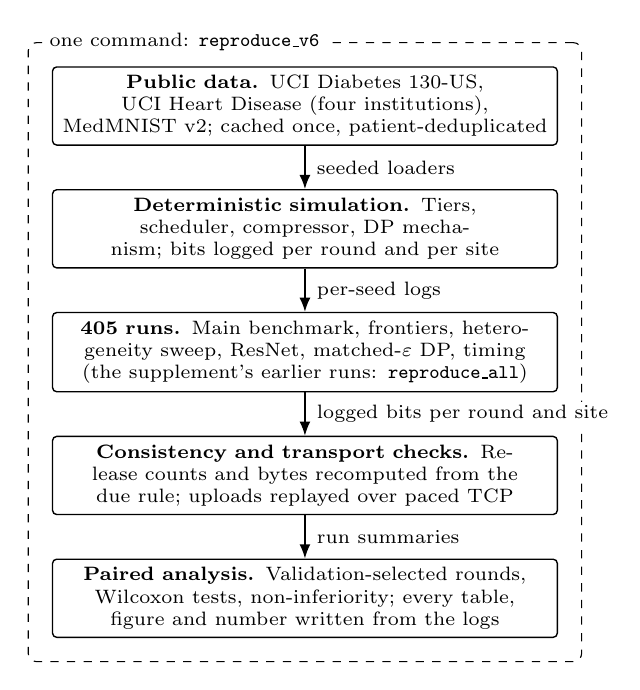
\begin{tikzpicture}[node distance=5.5mm, every node/.style={font=\scriptsize}]
\node[proc, text width=62mm] (d) {\textbf{Public data.} UCI Diabetes 130-US, UCI Heart Disease (four institutions), \mbox{MedMNIST v2}; cached once, patient-deduplicated};
\node[proc, text width=62mm, below=of d] (s) {\textbf{Deterministic simulation.} Tiers, scheduler, compressor, DP mechanism; bits logged per round and per site};
\node[proc, text width=62mm, below=of s] (r) {\textbf{405 runs.} Main benchmark, frontiers, heterogeneity sweep, ResNet, matched-$\varepsilon$ DP, timing (the supplement's earlier runs: \texttt{reproduce\_all})};
\node[proc, text width=62mm, below=of r] (e) {\textbf{Consistency and transport checks.} Release counts and bytes recomputed from the due rule; uploads replayed over paced TCP};
\node[proc, text width=62mm, below=of e] (a) {\textbf{Paired analysis.} Validation-selected rounds, Wilcoxon tests, non-inferiority; every table, figure and number written from the logs};
\draw[arr] (d) -- node[lab, right=1mm] {seeded loaders} (s);
\draw[arr] (s) -- node[lab, right=1mm] {per-seed logs} (r);
\draw[arr] (r) -- node[lab, right=1mm] {logged bits per round and site} (e);
\draw[arr] (e) -- node[lab, right=1mm] {run summaries} (a);
\begin{scope}[on background layer]
\node[grp, fit=(d)(s)(r)(e)(a), inner sep=3mm, label={[font=\scriptsize, fill=white, inner sep=2pt, anchor=west, xshift=2mm]north west:one command: \texttt{reproduce\_v6}}] {};
\end{scope}
\end{tikzpicture}
\caption{Study pipeline from the public data to every reported number. All stages run from one command, and the determinism check runs first.}
\label{fig:pipeline}
\end{figure}

\textbf{Metrics.} Each site's patients are split into training, validation and test sets (70/10/20\%, patient-grouped); $\mathcal V_k$ and $\mathcal T_k$ denote the last two. With $\mathrm{AUC}_k^{\mathcal T}(r)$ the AUROC of site $k$'s own model after round $r$ on $\mathcal T_k$, the personalised AUROC and the reported round are
\begin{equation}
\begin{gathered}
A^{\mathcal T}(r)=\frac{\sum_{k}|\mathcal T_k|\,\mathrm{AUC}^{\mathcal T}_k(r)}{\sum_{k}|\mathcal T_k|},\\
\hat r=\min\Big\{\arg\max_{r\le R}A^{\mathcal V}(r)\Big\},
\end{gathered}
\label{eq:metric}
\end{equation}
where $A^{\mathcal V}$ is the same average over the validation splits and sites whose split holds a single class are left out of each average, identically for every method. The primary metric is $A^{\mathcal T}(\hat r)$ with the bytes uploaded up to $\hat r$; test data never select anything. Secondary metrics are the mean of $A^{\mathcal T}$ over the last ten rounds, over the post-synchronisation rounds of the last twenty and at $r=R$, the ECE and Brier score~\cite{vancalster2019} before and after Platt scaling~\cite{platt1999} fitted on $\mathcal V_k$, and the worst-site AUROC $\min_k\mathrm{AUC}^{\mathcal T}_k(\hat r)$. Fig.~\ref{fig:pipeline} summarises the study.

\subsection{Problem Statement}
Given a quota $\rho$ on the payload fraction (\ref{eq:payload}), optionally a cap $\pi$ on the payload of any one round and a privacy budget $(\varepsilon^\star,\delta)$, the scheduler chooses intervals $\mathbf K$ and phases $\boldsymbol\phi$ for
\begin{equation}
\max_{\mathbf K,\boldsymbol\phi}\ A^{\mathcal T}(\hat r)\quad\text{s.t.}\quad\Pi_\infty(\mathbf K)\le\rho,\quad\hat P\le\pi,\quad\varepsilon(\mathbf K)\le\varepsilon^\star .
\label{eq:problem}
\end{equation}
A schedule succeeds if $A^{\mathcal T}(\hat r)$ is non-inferior to full-rate personalisation and at least that of the best uniform period at the same bytes. The objective is unknown before training, so Section~\ref{sec:method} optimises a surrogate. $\varepsilon(\mathbf K)$ is defined only for a schedule fixed before training, because the accountant charges only data-independent releases. Per-site non-inferiority is reported descriptively, not tested.

\section{Quota-Constrained Multi-Rate Scheduling}
\label{sec:method}

The scheduler separates \emph{what} is sent (tiers), \emph{when} (per-tier intervals chosen under the quota), \emph{how large} (an optional compressor) and \emph{how private} (the DP mechanism and its accountant). Fig.~\ref{fig:arch} shows the architecture. The server-side controller observes the received slices, the sites observe only the broadcast, and the link and the privacy mechanism sit between them.

\begin{figure*}[t]
\centering
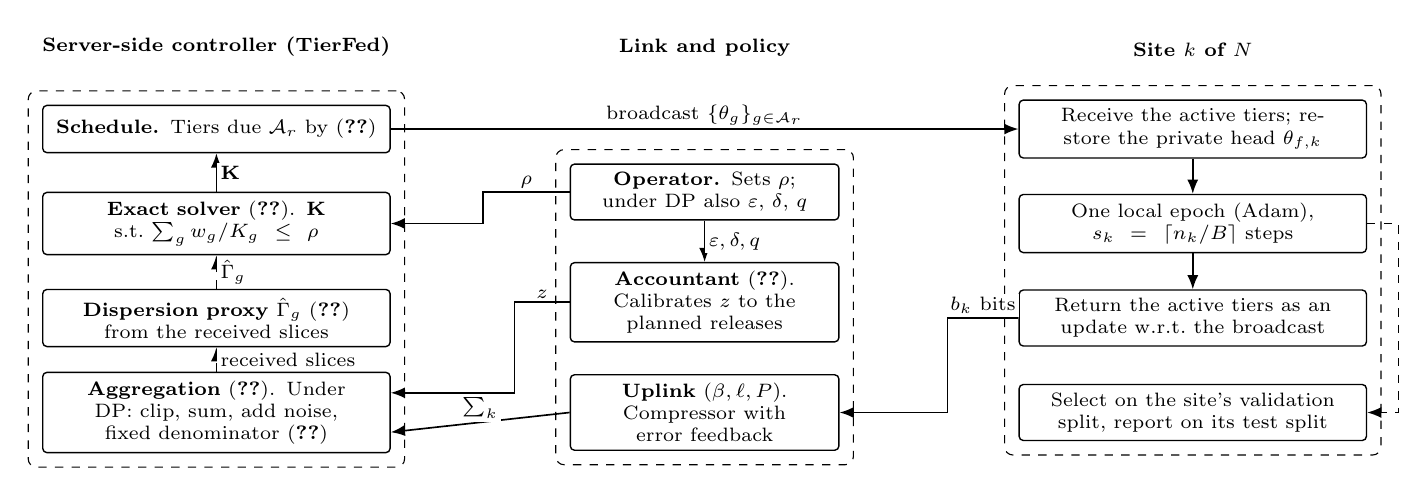
\begin{tikzpicture}[x=1mm,y=1mm]
\node[hdr] at (0,8) {Server-side controller (\tierfed{})};
\node[hdr] at (62,8) {Link and policy};
\node[hdr] at (124,8) {Site $k$ of $N$};
% server column
\node[srvbox, text width=42mm] (sched) at (0,0)   {\textbf{Schedule.} Tiers due $\mathcal A_r$ by (\ref{eq:due})};
\node[srvbox, text width=42mm] (solve) at (0,-12) {\textbf{Exact solver} (\ref{eq:ip}). $\mathbf K$ s.t.\ $\sum_g w_g/K_g\le\rho$};
\node[srvbox, text width=42mm] (disp)  at (0,-24) {\textbf{Dispersion proxy} $\Gh_g$ (\ref{eq:gammahat}) from the received slices};
\node[srvbox, text width=42mm] (agg)   at (0,-36) {\textbf{Aggregation} (\ref{eq:agg}). Under DP: clip, sum, add noise, fixed denominator (\ref{eq:dp})};
% link column
\node[lnkbox, text width=32mm] (op)   at (62,-8)  {\textbf{Operator.} Sets $\rho$; under DP also $\varepsilon$, $\delta$, $q$};
\node[lnkbox, text width=32mm] (acc)  at (62,-22) {\textbf{Accountant} (\ref{eq:rdp}). Calibrates $z$ to the planned releases};
\node[lnkbox, text width=32mm] (link) at (62,-36) {\textbf{Uplink} $(\beta,\ell,P)$. Compressor with error feedback};
% site column
\node[stebox, text width=42mm] (bcast) at (124,0)   {Receive the active tiers; restore the private head $\theta_{f,k}$};
\node[stebox, text width=42mm] (train) at (124,-12) {One local epoch (Adam), $s_k=\lceil n_k/B\rceil$ steps};
\node[stebox, text width=42mm] (ret)   at (124,-24) {Return the active tiers as an update w.r.t.\ the broadcast};
\node[stebox, text width=42mm] (eval)  at (124,-36) {Select on the site's validation split, report on its test split};
\begin{scope}[on background layer]
\node[grp, fit=(sched)(solve)(disp)(agg)] {};
\node[grp, fit=(op)(acc)(link)] {};
\node[grp, fit=(bcast)(train)(ret)(eval)] {};
\end{scope}
% data path down the round (solid)
\draw[arr] (sched.east) -- node[lab, above] {broadcast $\{\theta_g\}_{g\in\mathcal A_r}$} (bcast.west);
\draw[arr] (bcast.south) -- (train.north);
\draw[arr] (train.south) -- (ret.north);
\draw[arr] (ret.west) -- ++(-9,0) node[lab, above, pos=0.5] {$b_k$ bits} |- (link.east);
\draw[arr] (link.west) -- node[lab, above] {$\sum_k$} ([yshift=-2.5mm]agg.east);
% policy inputs (solid)
\draw[arr] (op.west) -- ++(-11,0) node[lab, above, pos=0.5] {$\rho$} |- (solve.east);
\draw[arr] (op.south) -- node[lab, right] {$\varepsilon,\delta,q$} (acc.north);
\draw[arr] (acc.west) -- ++(-7,0) node[lab, above, pos=0.5] {$z$} |- ([yshift=2.5mm]agg.east);
% measurements fed back (dashed)
\draw[meas] (agg.north) -- node[lab, right] {received slices} (disp.south);
\draw[meas] (disp.north) -- node[lab, right] {$\Gh_g$} (solve.south);
\draw[arr]  (solve.north) -- node[lab, right] {$\mathbf K$} (sched.south);
\draw[meas] (train.east) -- ++(4,0) |- (eval.east);
\end{tikzpicture}
\caption{Scheduler and environment. Solid arrows carry data and policy inputs; dashed arrows are measurements fed back. Under DP the dashed path from the received slices to the solver is cut and the schedule is planned before training (Section~\ref{sec:method-privacy}).}
\label{fig:arch}
\end{figure*}

\subsection{Dispersion Measurement}
\tierfed{} estimates the heterogeneity of each tier from the dispersion of the slices it receives. For tier $g$ with tensors $j\in g$,
\begin{equation}
\Gh_g^{(r)}=\frac{\sum_{j\in g}\frac1{|\mathcal S_r|}\sum_{k\in\mathcal S_r}\big\|\theta_{k,j}^{(r)}-\bar\theta_j^{(r)}\big\|_2^2}{\sum_{j\in g}\big\|\bar\theta_j^{(r)}\big\|_2^2+\xi_0},
\label{eq:gammahat}
\end{equation}
a scale-free ratio ($\xi_0=10^{-12}$) that makes tiers of different magnitude comparable. It exists only for tiers received in round $r$; otherwise the last value is carried forward. The received slices result from $m_g=(r-t_g)\,s$ local steps since the tier's last synchronisation $t_g$, and the standard drift lemma of local SGD~\cite{stich2019,khaled2020} bounds the expected numerator by a term of order $\eta^2(m_g\sigma_g^2+m_g^2\Gamma_g)$. $\Gh_g$ can therefore grow quadratically with the interval that produced it, so the controller partly measures its own decisions. The debiased proxy $\tilde\Gamma_g=\Gh_g/(r-t_g)^2$ removes the quadratic growth of the heterogeneity term; it is released as an option but not evaluated here.

\subsection{The Programme and Its Closed Form}
\emph{Bound.} The analysis concerns the shared backbone with the private heads frozen; the personalisation gap this introduces is measured empirically. Assume block-separable $L$-smoothness (the gradient of tier $g$ is $L$-Lipschitz in $\theta_g$ and does not depend on the other tiers; this ignores cross-tier coupling and is the main idealisation), unbiased stochastic gradients with per-tier variance $\sigma_g^2$, bounded per-tier heterogeneity $\frac1N\sum_k\|\nabla_gF_k(\theta)-\nabla_gF(\theta)\|^2\le\Gamma_g$, $F\ge F^\star$~\cite{stich2019,wang2021coop}, and the same number $s$ of local steps at every site. With unequal $s_k$, plain averaging converges towards a reweighted objective~\cite{wang2020fednova}; the experiments keep $s_k=\lceil n_k/B\rceil$ and do not normalise.
\begin{proposition}[Multi-rate local-SGD bound]
\label{prop:bound}
With local SGD of step size $\eta$ and tier $g$ averaged every $K_g$ rounds, there are absolute constants $c_0,c_1,c_2$ such that for $\eta\le c_0/(LK_{\max}s)$,
\begin{align}
\frac1R\sum_{r=1}^R\mathbb E\big\|\nabla F(\bar\theta_r)\big\|^2
&\le \frac{c_1(F(\bar\theta_1)-F^\star)}{\eta sR}+c_1\eta L\sum_g\frac{\sigma_g^2}{N}\notag\\
&\quad+c_2\,\eta^2L^2s^2\sum_g K_g^2\big(\Gamma_g+\sigma_g^2\big).
\label{eq:bound}
\end{align}
\end{proposition}
The proof applies the perturbed-iterate argument of~\cite{wang2021coop} blockwise (supplement, Section~S2). In the bound, a long interval is cheap only for a tier with small $\Gamma_g+\sigma_g^2$.

\emph{Programme.} Given a quota $\rho$ the controller solves
\begin{equation}
\mathbf K^\star=\arg\min_{K_g\in\{1,\dots,K_{\max}\}}\sum_{g\in\mathcal G_{\mathrm{sh}}}K_g^2\,\Gh_g\ \ \text{s.t.}\ \sum_{g\in\mathcal G_{\mathrm{sh}}}\frac{w_g}{K_g}\le\rho .
\label{eq:ip}
\end{equation}
It takes the last term of (\ref{eq:bound}) and replaces the unknown $\Gamma_g+\sigma_g^2$ by the measured proxy $\Gh_g$; the common factor $\eta^2L^2s^2$ does not change the minimiser. The proxy is not an estimate of $\Gamma_g+\sigma_g^2$: by the drift lemma its numerator after $m$ local steps is of order $\eta^2(m\sigma_g^2+m^2\Gamma_g)$, which weights the noise by $1/m$ rather than by one, and its denominator is the tier's own squared norm, a factor that differs between tiers. The programme is therefore a heuristic surrogate of the bound, and every statement below about (\ref{eq:ip}) concerns that surrogate. With the head private, $\mathcal G_{\mathrm{sh}}=\{\mathrm s,\mathrm m\}$ and $K_{\max}=8$, so the programme has 64 candidates and is solved by enumeration, with ties broken towards the denser schedule.

\begin{proposition}[Closed form and the value of differentiation]
\label{prop:cuberoot}
Let $\Gamma_g>0$, $w_g>0$, $\sum_gw_g=1$, and relax $K_g$ to the positive reals. Then (\ref{eq:ip}) has the unique minimiser
\begin{equation}
K_g^\star=\Big(\frac{w_g}{\Gamma_g}\Big)^{1/3}\frac{S}{\rho},\qquad S=\sum_hw_h^{2/3}\Gamma_h^{1/3},
\label{eq:cuberoot}
\end{equation}
with value $J^\star=S^3/\rho^2$. The uniform interval $K=1/\rho$ costs $J_{\mathrm u}=\sum_g\Gamma_g/\rho^2$, and
\begin{equation}
\Psi=1-\frac{J^\star}{J_{\mathrm u}}=1-\frac{S^3}{\sum_g\Gamma_g}\in[0,1),
\label{eq:psi}
\end{equation}
with $\Psi=0$ if and only if $w_g/\Gamma_g$ is equal for all tiers. When $1/\rho$ is an integer, no integer schedule lowers the objective of (\ref{eq:ip}) below that of the uniform period by more than the fraction $\Psi$.
\end{proposition}
The proof (supplement, Section~S2) applies the KKT conditions of the convex programme, H\"older's inequality with exponents $3/2$ and $3$ for $\Psi\ge0$, and the integer feasibility of $K=1/\rho$. Two consequences shape the evaluation. The interval ratio $K_a/K_b=(w_a\Gamma_b/w_b\Gamma_a)^{1/3}$ compresses differences, since a factor of eight in payload-to-dispersion ratio is needed for a factor of two in interval, so tiers with similar ratios collapse onto one interval after rounding. And Proposition~\ref{prop:cuberoot} holds for any positive weights, so it applies exactly to (\ref{eq:ip}) with $\Gh_g$ in place of $\Gamma_g$. $\Psi$ is invariant to a factor common to all tiers, such as the interval when every tier has been synchronised every round; evaluated on $\Gh_g$ at the end of warm-up, it states before any sparse round how much a per-tier schedule can reduce the surrogate below a uniform one. It does not state how much accuracy that reduction buys.

\subsection{Schedule Rule, Phases and the Quota}
Rounds are indexed $r=1,\dots,R$. The first $T_w$ rounds synchronise every shared tier, and thereafter tier $g$ is due when
\begin{equation}
\mathcal A_r=\begin{cases}\mathcal G_{\mathrm{sh}}, & r\le T_w,\\ \{g:\ (r-T_w-\phi_g)\bmod K_g=0\}, & r>T_w,\end{cases}
\label{eq:due}
\end{equation}
with phase $\phi_g=0$ unless staggered. The fixed periods, the DP planner and the accountant all use this one rule, and the consistency check of Section~\ref{sec:results-check} recomputes every release from it. Adaptive \tierfed{} sends tier $g$ when $r-t_g\ge K_g$, which coincides with (\ref{eq:due}) whenever $\mathbf K$ is constant after warm-up. $T_w=5$ and $K_{\max}=8$ throughout. Fig.~\ref{fig:round} shows one server round.

\emph{Phases and the peak.} A mean quota does not bound the payload $P_r$ of a single round, because aligned tiers coincide and send the full shared payload. Two tiers with phases $\phi_a,\phi_b$ are never due in the same round if and only if $\phi_a-\phi_b\not\equiv0\pmod{\gcd(K_a,K_b)}$ (Chinese remainder theorem), so with $\gcd\ge2$ the offset $\lfloor\gcd/2\rfloor$ separates them and bounds the post-warm-up peak by $\max_gw_g$ at the same long-run payload fraction $\Pi_\infty$ (over a finite horizon $\Pi_R$ can differ slightly, because the phase moves which syncs fall inside it); with co-prime intervals no phase helps. The staggered variant adds $\max_{r>T_w}P_r\le\pi$ to (\ref{eq:ip}) and checks it over one hyper-period $\mathrm{lcm}(\mathbf K)$. A full-rate warm-up still sends the whole payload, so the warm-up rounds can be sent at eight bits.

\emph{The quota.} Solving (\ref{eq:ip}) with $\rho$ bounds $\Pi_\infty$ of (\ref{eq:payload}), not the realised $\Pi_R$: a warm-up of $T_w$ rounds at payload fraction $c_w$ adds $T_w(c_w-\Pi_\infty)/R$ to the realised fraction. A quota over all rounds is met by solving with $\rho'=(\rho R-c_wT_w)/(R-T_w)$; both forms are reported, and the realised $\Pi_R$ is read from the logs.

\begin{figure}[t]
\centering
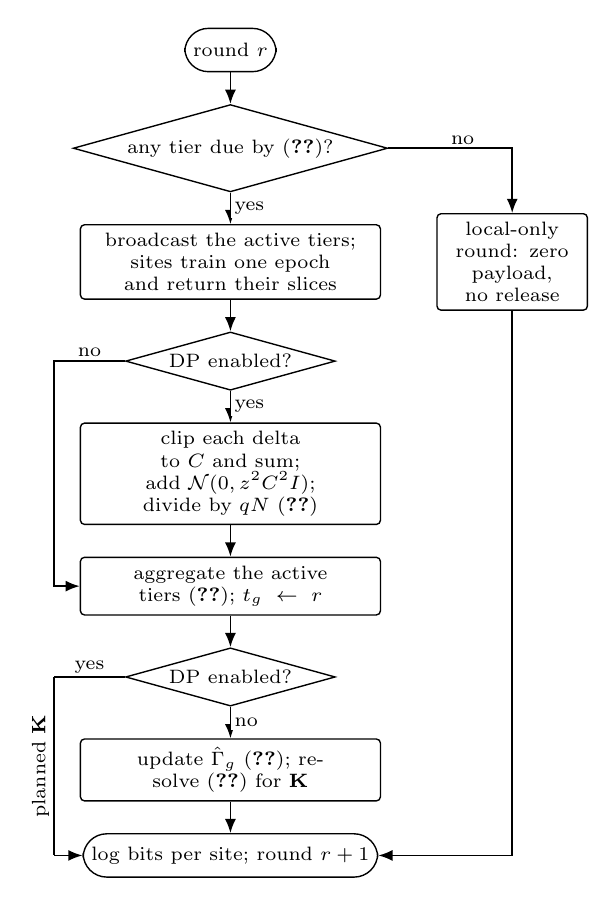
\begin{tikzpicture}[node distance=4mm and 6mm, every node/.style={font=\scriptsize}]
\node[term] (start) {round $r$};
\node[dec, below=of start] (due) {any tier due by (\ref{eq:due})?};
\node[proc, text width=36mm, below=of due] (bc) {broadcast the active tiers; sites train one epoch and return their slices};
\node[dec, below=of bc] (dp) {DP enabled?};
\node[proc, text width=36mm, below=of dp] (priv) {clip each delta to $C$ and sum;\\ add $\mathcal N(0,z^2C^2I)$;\\ divide by $qN$ (\ref{eq:dp})};
\node[proc, text width=36mm, below=of priv] (ag) {aggregate the active tiers (\ref{eq:agg}); $t_g\leftarrow r$};
\node[dec, below=of ag] (dp2) {DP enabled?};
\node[proc, text width=36mm, below=of dp2] (upd) {update $\Gh_g$ (\ref{eq:gammahat}); re-solve (\ref{eq:ip}) for $\mathbf K$};
\node[term, below=of upd] (next) {log bits per site; round $r+1$};
\node[proc, text width=17mm, right=7mm of bc] (local) {local-only round: zero payload, no release};
\draw[arr] (start) -- (due);
\draw[arr] (due) -- node[lab, right] {yes} (bc);
\draw[arr] (due.east) -| node[lab, above, pos=0.3] {no} (local);
\draw[arr] (local.south) |- (next.east);
\draw[arr] (bc) -- (dp);
\draw[arr] (dp) -- node[lab, right] {yes} (priv);
\draw[arr] (dp.west) -- ++(-9mm,0) node[lab, above, pos=0.5] {no} |- (ag.west);
\draw[arr] (priv) -- (ag);
\draw[arr] (ag) -- (dp2);
\draw[arr] (dp2) -- node[lab, right] {no} (upd);
\coordinate (k1) at ($(dp2.west)+(-9mm,0)$);
\coordinate (k2) at (k1 |- next.west);
\draw[line width=0.6pt] (dp2.west) -- node[lab, above] {yes} (k1);
\draw[line width=0.6pt] (k1) -- node[midway, rotate=90, anchor=south, font=\scriptsize, inner sep=1.5pt] {planned $\mathbf K$} (k2);
\draw[arr] (k2) -- (next.west);
\draw[arr] (upd) -- (next);
\end{tikzpicture}
\caption{One server round. Under DP the schedule is fixed before training and the dispersion feedback is never computed from the private slices.}
\label{fig:round}
\end{figure}

\emph{Compression.} A compressor that emits a fraction $\kappa\in(0,1]$ of the float32 bits multiplies the upload, $B=R\,|\mathcal S|\,\Pi_R(\mathbf K)\,\kappa\,32\,d_{\mathrm{sh}}$ bits for $d_{\mathrm{sh}}$ shared parameters; it acts on each site's update relative to the broadcast, with error feedback, and the bits it emits are counted.

\subsection{Privacy: Threat Model, Mechanism and Eligible Schedules}
\label{sec:method-privacy}
\emph{Threat model.} Sites send their updates over TLS to an aggregator that is trusted to apply the mechanism and sees raw updates, as in central DP-FedAvg~\cite{mcmahan2018dp}; central DP protects the released aggregates against their consumers, the other sites among them. A passive network observer cannot read the payloads but sees when each site transmits and how many bytes, which is exactly the schedule, so a schedule that depends on client data leaks even under encryption. Secure aggregation with distributed noise~\cite{kairouz2021ddg} would remove the trust in the aggregator but not this metadata; poisoning is out of scope.

\emph{Mechanism.} Each round every site joins the cohort $\mathcal S_r$ independently with probability $q$; $q=1$, full participation, is the primary cross-silo setting and $q<1$ a sensitivity analysis. The server clips every participating site's returned delta and adds noise to the sum before dividing by the \emph{fixed} expected cohort size,
\begin{equation}
\tilde\Delta=\frac1{qN}\Big(\sum_{k\in\mathcal S_r}\Delta_k\min\big(1,\tfrac{C}{\|\Delta_k\|_2}\big)+\mathcal N(0,z^2C^2I)\Big),
\label{eq:dp}
\end{equation}
the fixed-denominator DP-FedAvg estimator~\cite{mcmahan2018dp}, so that adding or removing one site changes the sum by at most $C$ in $\ell_2$ and the denominator reveals nothing about the realised cohort; a planned release whose cohort is empty still adds noise. The server applies it to every method identically.

\emph{Accountant.} Over the $R_{\mathrm{tx}}$ planned releases the R\'enyi DP of the Poisson-subsampled Gaussian mechanism is composed at integer orders~\cite{mironov2019sgm},
\begin{align}
\varepsilon_\alpha&=\frac{R_{\mathrm{tx}}}{\alpha-1}\log\sum_{k=0}^{\alpha}\binom{\alpha}{k}(1-q)^{\alpha-k}q^ke^{\frac{k^2-k}{2z^2}},\notag\\
\varepsilon&=\min_\alpha\Big\{\varepsilon_\alpha+\frac{\log(1/\delta)}{\alpha-1}\Big\},
\label{eq:rdp}
\end{align}
with $\delta=10^{-5}$; for $q=1$ this reduces to $R_{\mathrm{tx}}\alpha/(2z^2)$~\cite{mironov2017}. The implementation reproduces the TensorFlow-Privacy MNIST reference ($\varepsilon\approx3.0$) and the $q=1$ closed form as unit tests. At $q=1$ the exact privacy of $R_{\mathrm{tx}}$ Gaussian releases is $\mu$-Gaussian DP with $\mu=\sqrt{R_{\mathrm{tx}}}/z$~\cite{dong2022gdp}, whose $(\varepsilon,\delta)$ curve~\cite{balle2018} is
\begin{equation}
\delta(\varepsilon)=\Phi\Big(-\frac{\varepsilon}{\mu}+\frac{\mu}{2}\Big)-e^{\varepsilon}\,\Phi\Big(-\frac{\varepsilon}{\mu}-\frac{\mu}{2}\Big),
\label{eq:gdp}
\end{equation}
with $\Phi$ the standard normal distribution function. Both accountants depend on $R_{\mathrm{tx}}$ only through $R_{\mathrm{tx}}/z^2$, so the exact one lowers every method's noise multiplier by the same factor, 13--24\% for $\varepsilon^\star$ from 8 to 1. The comparison at matched $\varepsilon$ is therefore unchanged, and every reported $\varepsilon$ is an upper bound; $z$ is calibrated to each method's own release count by bisection on (\ref{eq:rdp}).

\emph{Which schedules are covered.} The accountant covers a release only if the decision to release does not depend on the private data. This holds for FedAvg, FedProx, FedPer, local training, a fixed period and the planner below, whose release rounds are fixed before training, and not for adaptive \tierfed{}, AdaComm, LAG or FedLAMA, whose schedules are functions of client updates or losses; the released code refuses to run them under DP. Privacy filters and odometers~\cite{rogers2016odometer} and the sparse vector technique~\cite{lyu2017svt} charge for data-dependent release decisions; FL schedulers take such decisions without charging for them. DP-FTRL~\cite{kairouz2021ftrl} and matrix-factorisation mechanisms~\cite{choquette2023banded} suit full participation but also need data-independent release rounds; they are not evaluated.

\emph{Planning under a privacy budget (\tierfed{}-DP).} A planner that respects the accountant chooses $\mathbf K$ before training from public quantities only, $(\varepsilon^\star,\delta)$, $q$, $R$, $T_w$, $w_g$ and $\rho$. For each candidate it computes the release set of (\ref{eq:due}), the smallest $z(\mathbf K)$ that keeps those releases $(\varepsilon^\star,\delta)$-DP, and minimises
\begin{equation}
J(\mathbf K)=\frac{\sum_g w_gK_g^2}{K_{\max}^2}+\lambda\,\frac{\sum_{r}P_r(\mathbf K)\,z(\mathbf K)^2}{\sum_{r}P_r(\mathbf 1)\,z(\mathbf 1)^2},
\label{eq:jdp}
\end{equation}
the drift term of (\ref{eq:bound}) under a flat heterogeneity prior plus the injected noise energy, each normalised by its worst case ($\lambda=1$); fewer releases need less noise but drift more. Under the flat prior, $\Gamma_g\propto w_g$ and Proposition~\ref{prop:cuberoot} gives $\Psi=0$, so the planner can only choose equal intervals; it is evaluated as an ablation, not claimed as a contribution.

\section{Experimental Setup}
\label{sec:setup}
Every method is run under the protocol of Section~\ref{sec:system} on the same seeds and splits, and every number is read from the logs. This section lists the experiment families, the baselines and bounds, the privacy and timing experiments, and the statistics that decide each comparison.

\begin{table}[t]
\caption{Experiment families of the main protocol, counted from the logs: data and sites, configurations, seeds and runs}
\label{tab:families}
\centering\footnotesize
\fit{\begin{tabular}{@{}llccc@{}}
\toprule
Family & Data, sites & Methods & Seeds & Runs\\
\midrule
Main comparison & 20 specialty sites & 13 & 10 & 130\\
Reference bounds & pooled / per site & 2 & 10 & 20\\
Iso-byte frontier & 20 specialty sites & 8 & 5 & 40\\
Peak-aware variants & 20 specialty sites & 3 & 5 & 15\\
Label-skew sweep & Dirichlet $\alpha\in\{0.1,0.3,1,10\}$ & 5 & 5 & 100\\
ResNet backbone & 20 specialty sites & 5 & 6 & 30\\
Matched-$\varepsilon$ DP ($q=1$) & 20 specialty sites & 5 & 6 & 30\\
Timing side channel & clean / shifted site 0 & 4 & 5 & 40\\
\bottomrule
\end{tabular}
}
\end{table}

\textbf{Experiment families.} Table~\ref{tab:families} lists the 405 runs: the main comparison; the iso-byte frontier, each method with its own knob swept; the label-skew sweep and the ResNet backbone, which test the regimes to which Proposition~\ref{prop:cuberoot} points; matched-$\varepsilon$ DP and the timing side channel for the privacy claims; and the peak-aware variants. Results of the earlier final-round protocol (compression, real institutions, imaging, scaling, a wide model) are in the supplement.

\textbf{Baselines and bounds.} \emph{Full rate:} FedAvg~\cite{mcmahan2017}, FedProx~\cite{li2020fedprox} and FedPer~\cite{arivazhagan2019}, the reference for the non-inferiority tests. \emph{Round-sparse:} AdaComm~\cite{wang2019adacomm}, LAG~\cite{chen2018lag} with sample weighting and, for comparison with earlier versions, with the equal weights used there, a FedLAMA-style per-layer interval rule reimplemented from its published description~\cite{lee2023fedlama}, and fixed periods on (\ref{eq:due}) with the same private head and warm-up as \tierfed{}. \emph{Bounds:} local training without communication, a centralised MLP trained on the pooled training splits of all sites for the same number of passes, and gradient boosting~\cite{ke2017lightgbm}; all three are scored on the same per-site test splits with the round, epoch or iteration chosen on validation. SCAFFOLD, whose control variates fit Adam poorly, is reported with SGD in the supplement.

\textbf{Differential privacy.} FedPer, fixed periods $K=4$ and $K=8$, one-shot federation (no warm-up, one release in round $R$, after a data-independent broadcast of the initial model) and the planner run at $\varepsilon^\star=4$, $\delta=10^{-5}$, $q=1$, $C=1$, each with $z$ calibrated to its own release count. Local training is the $\varepsilon=0$ reference on the same splits. The $q<1$ sweeps over $\varepsilon^\star\in\{1,2,4,8\}$ on 20 and 100 sites are in the supplement.

\textbf{Timing side channel.} One target site holds half of its labels flipped (shifted world) or none (clean world). A passive observer sees which rounds carry traffic and how many bytes each site sends, and reduces each run to an observable $o$: the rounds with traffic, the target's rounds, the target's bytes or the bytes of all sites. Its power is the Mann--Whitney AUC over the $n_1$ shifted and $n_0$ clean runs,
\begin{equation}
\mathrm{AUC}=\frac1{n_1n_0}\sum_{i=1}^{n_1}\sum_{j=1}^{n_0}\Big(\mathbb 1\big[o^{(1)}_i>o^{(0)}_j\big]+\tfrac12\,\mathbb 1\big[o^{(1)}_i=o^{(0)}_j\big]\Big),
\label{eq:auc}
\end{equation}
where 0.5 means that the schedule reveals nothing; an AUC of at least 0.75 on any observable is reported as a leak.

\textbf{Statistics.} All comparisons are paired across seeds. Two primary contrasts were fixed in the code before the runs, with the metric and both thresholds: \tierfed{} against FedPer, and \tierfed{} against the best uniform period at matched bytes. With $\mathcal U$ the uniform periods run in a setting, $B$ the mean upload and $\bar A^{\mathcal V}$ the mean validation AUROC at $\hat r$, that period and the gain over it are
\begin{equation}
\begin{gathered}
K_{\mathrm u}=\arg\max_{K\in\mathcal U:\,B_K\le1.05\,B_{\mathrm{TF}}}\bar A^{\mathcal V}_K,\\
\Delta_{\mathrm u}=\frac1S\sum_{s=1}^{S}\big(A^{\mathcal T}_{\mathrm{TF},s}-A^{\mathcal T}_{K_{\mathrm u},s}\big),
\end{gathered}
\label{eq:gate}
\end{equation}
over the $S$ seeds both share; every other comparison is exploratory. Tests are two-sided Wilcoxon signed-rank tests and intervals are percentile bootstrap intervals over seeds. The gate first required a Holm-corrected $p<0.05$, which 5 or 6 seeds cannot reach, so $\Delta_{\mathrm u}$ is read from its interval: a setting counts as a gain only when the 95\% interval excludes zero and $\Delta_{\mathrm u}\ge0.005$ AUROC; no setting passes either rule. A difference below 0.005 is not called relevant, whatever its $p$. Non-inferiority to FedPer is tested one-sided,
\begin{equation}
H_0:\ \mathbb E[d]\le-\Delta_{\mathrm{NI}},\qquad d=A^{\mathcal T}_{\text{method}}(\hat r)-A^{\mathcal T}_{\text{FedPer}}(\hat r),
\label{eq:ni}
\end{equation}
by the signed-rank test on $d+\Delta_{\mathrm{NI}}$ at $\Delta_{\mathrm{NI}}=0.01$ and, as a sensitivity margin, 0.005. Repeated runs are bit-identical on one machine. On a second machine every data-independent schedule sends the same bytes, but the AUROC of a single run can move by up to 0.0893 (Section~\ref{sec:results-check}), so every comparison is computed within one machine.

\section{Results}
\label{sec:results}

The results proceed from the protocol checks to the main comparison, the conditions under which per-tier scheduling can pay, the cost on constrained links and privacy. Unless stated otherwise, values are means over seeds on Diabetes with the MLP and the specialty sites, $p$-values are from paired Wilcoxon tests, and tables S-$n$ are in the supplement.

\subsection{Protocol Checks}
\label{sec:results-check}
The consistency check recomputes, from the stated rules, the transmitting rounds of every data-independent schedule, the bits of every uncompressed round with full participation and the releases charged by the accountant, over all 2,218 logs of this article; it finds 0 mismatches in 977 schedule, 872 byte and 230 accountant checks. Of the 130 label-skew and timing runs repeated on a Windows laptop (all main-protocol runs used one Linux machine), every data-independent schedule sends the same bytes in every round, and 29 of the 40 adaptive runs do, the rest differing by up to 2.9\% because their decisions read client data. The AUROC at the selected round moves by a median of 0.0004 and at most 0.0893, at strong label skew: on a flat validation curve a small numerical difference selects another round (36 runs). The gate decision and the leak verdicts are unchanged. Because the selected round can move, both primary contrasts are repeated under a smoothed rule (the round that maximises the trailing three-round mean of $A^{\mathcal V}$) and under the mean of the last ten rounds (supplement, Section~S4). No reading puts \tierfed{} ahead of the best uniform period by 0.005 in any setting. Its parity with FedPer is less robust. Under the smoothed rule it trails FedPer by \ensuremath{-}0.0125 [\ensuremath{-}0.0168, \ensuremath{-}0.0090] at $\alpha=10$ and by \ensuremath{-}0.0071 [\ensuremath{-}0.0116, \ensuremath{-}0.0030] on the ResNet, because the argmax rule can read the peak that follows a synchronisation.

\begin{table*}[t]
\caption{Main comparison on the 20 specialty sites (MLP, 10 seeds): $A^{\mathcal T}(\hat r)$ with bootstrap 95\% interval; upload over 60 rounds and up to $\hat r$; mean over the last ten rounds and over the post-synchronisation rounds of the last twenty (Phase); final model after three local epochs (+FT 3); ECE without and with Platt scaling; worst-site AUROC; $\Delta$ and $p$ against FedPer. $\equiv$: the two schedules send the same tiers in every round and give identical runs}
\label{tab:main}
\centering\footnotesize
\fit{\begin{tabular}{@{}lcccccccccc@{}}
\toprule
Method & AUROC, val.-selected [95\% CI] & MB & MB to sel. & Last 10 & Phase & +FT 3 & ECE raw/Platt & Worst site & $\Delta$ FedPer & $p$\\
\midrule
Local only & 0.6145 [0.6090, 0.6204] & 0.0 & 0.0 & 0.5557 & 0.5564 & 0.5548 & 0.363/0.023 & 0.431 & \ensuremath{-}0.0239 & 0.002\\
FedAvg & 0.6391 [0.6341, 0.6448] & 218.4 & 50.6 & 0.6230 & 0.6252 & 0.6069 & 0.365/0.024 & 0.468 & \ensuremath{+}0.0006 & 0.064\\
FedProx & 0.6391 [0.6348, 0.6438] & 218.4 & 77.9 & 0.6283 & 0.6306 & 0.6108 & 0.361/0.025 & 0.488 & \ensuremath{+}0.0006 & 0.432\\
FedPer & 0.6385 [0.6337, 0.6437] & 217.8 & 63.2 & 0.6261 & 0.6279 & 0.6083 & 0.367/0.024 & 0.468 & -- & --\\
FedLAMA-style & 0.6396 [0.6344, 0.6457] & 154.1 & 49.4 & 0.6314 & 0.6329 & 0.6119 & 0.363/0.024 & 0.476 & \ensuremath{+}0.0011 & 0.131\\
AdaComm & 0.6329 [0.6273, 0.6391] & 29.1 & 27.7 & 0.6302 & 0.6300 & 0.6234 & 0.363/0.023 & 0.463 & \ensuremath{-}0.0056 & 0.004\\
LAG, equal weights & 0.6373 [0.6327, 0.6417] & 218.4 & 116.9 & 0.6344 & 0.6350 & 0.6218 & 0.362/0.024 & 0.480 & \ensuremath{-}0.0012 & 0.492\\
LAG & 0.6395 [0.6342, 0.6458] & 218.4 & 44.4 & 0.6237 & 0.6259 & 0.6079 & 0.366/0.024 & 0.470 & \ensuremath{+}0.0011 & 0.064\\
Fixed (8,8) & 0.6372 [0.6317, 0.6440] & 39.9 & 35.9 & 0.6280 & 0.6379 & 0.6003 & 0.363/0.024 & 0.457 & \ensuremath{-}0.0013 & 0.275\\
\tierfed{} $\equiv$ Fixed (4,4) & 0.6377 [0.6327, 0.6440] & 65.3 & 45.7 & 0.6346 & 0.6396 & 0.6122 & 0.361/0.024 & 0.463 & \ensuremath{-}0.0007 & 0.557\\
\tierfed{}, staggered $\equiv$ Fixed (4,4), staggered & 0.6353 [0.6309, 0.6399] & 67.0 & 40.2 & 0.6289 & 0.6327 & 0.6112 & 0.359/0.024 & 0.447 & \ensuremath{-}0.0032 & 0.049\\
Centralised MLP & 0.6435 [0.6373, 0.6506] & -- & -- & 0.5936 & -- & -- & 0.363/-- & -- & \ensuremath{+}0.0050 & 0.004\\
Gradient boosting & 0.6413 [0.6348, 0.6491] & -- & -- & 0.6272 & -- & -- & 0.019/-- & -- & \ensuremath{+}0.0029 & 0.160\\
\bottomrule
\end{tabular}
}
\end{table*}

\subsection{Main Comparison}
\label{sec:results-main}
At the validation-selected round the federated methods are close (Table~\ref{tab:main}). FedPer reaches 0.6385, and apart from AdaComm no method differs from it by more than 0.0032 AUROC, below the 0.005 that this study calls relevant (largest difference: Fixed (4,4), staggered, $p=0.049$). AdaComm is lower by a relevant margin, \ensuremath{-}0.0056 ($p=0.004$), at 29.1 against 217.8~MB, and local training by \ensuremath{-}0.0239 ($p=0.002$), so federation helps on this task.
On this benchmark \tierfed{} chooses $\mathbf K=(4,4)$ in every seed, and after warm-up its schedule is that of the fixed period $(4,4)$ round for round, so the two runs are identical and Table~\ref{tab:main} shows them as one row. %
This is what Proposition~\ref{prop:cuberoot} predicts: at the end of warm-up $\Psi=0.1$\%, so no per-tier schedule can improve the drift surrogate over a uniform period by more than that fraction. \tierfed{} is non-inferior to FedPer at $\Delta_{\mathrm{NI}}=0.01$ ($p<10^{-3}$) and at 0.005 ($p=0.007$), with 65.3 against 217.8~MB over 60 rounds; AdaComm, at 29.1~MB, is non-inferior at 0.01 ($p=0.007$) but not at 0.005 ($p=0.615$).

\begin{figure*}[t]
\centering\fig{fig_dynamics}{\textwidth}
\caption{Training on the specialty sites (MLP, 10 seeds). (a) $A^{\mathcal T}(r)$, mean and 95\% interval; dots: mean $\hat r$; the \tierfed{} curve is also that of Fixed $(4,4)$, and LAG coincides with FedPer. (b) Cumulative upload. (c) Upload of site~0 per round as a share of its shared payload, aligned against staggered $(4,4)$ (seed 42, rounds 1--21; rounds 1--5: warm-up).}
\label{fig:dyn}
\end{figure*}

The final-round lead of the sparse schedules, reported in an earlier version of this work (supplement, Section~S1), is a property of the round at which they are read. Full-rate training passes its best validation round early (round 17 on average, against 36 for \tierfed{}; dots in Fig.~\ref{fig:dyn}(a)) and then overfits, while a sparse schedule climbs in a sawtooth that peaks after each synchronisation. Over the last ten rounds the sparse schedules are therefore ahead (\tierfed{} 0.6346, FedPer 0.6261); at the validation-selected round the lead disappears, while the upload gap of Fig.~\ref{fig:dyn}(b) remains. Fine-tuning each site's final model for three local epochs lowers the AUROC of every method, by 0.0006 to 0.0169, so the late-round lead is not local adaptation either. Sparse synchronisation overfits later. LAG's earlier lead came from its weighting. Its final-round AUROC is 0.6337 with the equal weights used there and 0.6212 with sample weights, level with FedAvg (0.6199); at its default threshold it never skips an upload.

AUPRC follows the same pattern (FedPer 0.177, \tierfed{} 0.174, local training 0.155, prevalence baseline 0.09). Inverse-frequency class weighting shifts every method's scores, so raw ECE is 0.359--0.367; Platt scaling on each site's validation split lowers it to 0.023--0.025 for every method at no communication cost. The worst site's AUROC is 0.431--0.488: the sample-weighted mean hides sites at which no method is useful.

\begin{table}[t]
\caption{\tierfed{} against every baseline of Table~\ref{tab:main}, paired over 10 seeds: AUROC difference with bootstrap 95\% interval, Holm-corrected Wilcoxon $p$, seeds on which \tierfed{} is strictly higher, and upload difference (MB). Fixed (4,4) is identical to \tierfed{} and is not listed}
\label{tab:paired}
\centering\footnotesize
\fit{\begin{tabular}{@{}lcccc@{}}
\toprule
\tierfed{} vs. & $\Delta$AUROC [95\% CI] & $p_{\mathrm{Holm}}$ & Higher & $\Delta$MB\\
\midrule
Local only & \ensuremath{+}0.0232 [\ensuremath{+}0.0187, \ensuremath{+}0.0272] & 0.023 & 10/10 & \ensuremath{+}65.3\\
FedAvg & \ensuremath{-}0.0014 [\ensuremath{-}0.0042, \ensuremath{+}0.0012] & 1.000 & 4/10 & \ensuremath{-}153.1\\
FedProx & \ensuremath{-}0.0014 [\ensuremath{-}0.0047, \ensuremath{+}0.0023] & 1.000 & 2/10 & \ensuremath{-}153.1\\
FedPer & \ensuremath{-}0.0007 [\ensuremath{-}0.0033, \ensuremath{+}0.0018] & 1.000 & 4/10 & \ensuremath{-}152.5\\
FedLAMA-style & \ensuremath{-}0.0019 [\ensuremath{-}0.0044, \ensuremath{+}0.0002] & 1.000 & 3/10 & \ensuremath{-}88.7\\
AdaComm & \ensuremath{+}0.0048 [\ensuremath{+}0.0022, \ensuremath{+}0.0076] & 0.107 & 9/10 & \ensuremath{+}36.2\\
LAG, equal weights & \ensuremath{+}0.0005 [\ensuremath{-}0.0028, \ensuremath{+}0.0043] & 1.000 & 4/10 & \ensuremath{-}153.1\\
LAG & \ensuremath{-}0.0018 [\ensuremath{-}0.0044, \ensuremath{+}0.0004] & 1.000 & 4/10 & \ensuremath{-}153.1\\
Fixed (8,8) & \ensuremath{+}0.0005 [\ensuremath{-}0.0015, \ensuremath{+}0.0023] & 1.000 & 7/10 & \ensuremath{+}25.4\\
Staggered (4,4) & \ensuremath{+}0.0024 [\ensuremath{+}0.0000, \ensuremath{+}0.0052] & 1.000 & 7/10 & \ensuremath{-}1.6\\
\bottomrule
\end{tabular}
}
\end{table}

Table~\ref{tab:paired} compares \tierfed{} with each baseline directly. It is above local training on 10/10 seeds, by \ensuremath{+}0.0232 [\ensuremath{+}0.0187, \ensuremath{+}0.0272] ($p_{\mathrm{Holm}}=0.023$), and above AdaComm on 9/10, by \ensuremath{+}0.0048 [\ensuremath{+}0.0022, \ensuremath{+}0.0076] ($p_{\mathrm{Holm}}=0.107$) while sending 36.2~MB more. Against every other federated method the difference is at most 0.0024 in absolute value and no Holm-corrected test is significant.

\subsection{When Does Per-Tier Scheduling Pay?}
\label{sec:results-arch}

\begin{figure*}[t]
\centering\fig{fig_au}{\textwidth}
\caption{(a) $A^{\mathcal T}(\hat r)$ against total upload, each method with its own knob swept (mean, 95\% interval; grey: local training, centralised MLP, gradient boosting). (b) $A^{\mathcal T}(\hat r)$ against Dirichlet label skew, series offset horizontally so that equal values stay visible; dotted: local training. (c) Gain $\Delta_{\mathrm u}$ of (\ref{eq:gate}) against $\Psi$ at the end of warm-up, one point per setting. (d) Window violations $v(W)$ on the 5-Mbit/s link against the window relative to the full-payload upload time; identical schedules coincide.}
\label{fig:au}
\end{figure*}

\begin{table*}[t]
\caption{Primary contrast (\ref{eq:gate}): \tierfed{} ($\rho=0.25$) against the best uniform period at matched bytes. $\Psi$ at the end of warm-up; $\mathbf K$: \tierfed{}'s intervals (slow, medium) in the first round after warm-up, most frequent over seeds; MB over 60 rounds; gain $\Delta_{\mathrm u}$ with bootstrap 95\% interval and Wilcoxon $p$. ``Identical runs'': \tierfed{} chose the intervals of the best uniform period and sent the same tiers in every round}
\label{tab:gate}
\centering\footnotesize
\fit{\begin{tabular}{@{}lcccccccccc@{}}
\toprule
Setting & $\Psi$ (\%) & $\mathbf K$ & \tierfed{} & MB & Best uniform & AUROC & MB & Gain [95\% CI] & $p$ & Seeds\\
\midrule
Specialty sites & 0.1 & (4,4) & 0.6377 & 65 & $K=4$ & 0.6377 & 65 & identical runs & -- & 10\\
Dirichlet $\alpha=0.1$ & 0.2 & (4,4) & 0.5858 & 52 & $K=8$ & 0.5971 & 31 & \ensuremath{-}0.0113 [\ensuremath{-}0.0270, \ensuremath{+}0.0040] & 0.625 & 5\\
Dirichlet $\alpha=0.3$ & 0.7 & (4,4) & 0.6003 & 65 & $K=4$ & 0.6003 & 65 & identical runs & -- & 5\\
Dirichlet $\alpha=1$ & 2.2 & (4,4) & 0.6176 & 65 & $K=4$ & 0.6176 & 65 & identical runs & -- & 5\\
Dirichlet $\alpha=10$ & 0.2 & (4,4) & 0.6445 & 65 & $K=4$ & 0.6445 & 65 & identical runs & -- & 5\\
ResNet backbone & 71.4 & (1,5) & 0.6413 & 604 & $K=4$ & 0.6434 & 602 & \ensuremath{-}0.0020 [\ensuremath{-}0.0072, \ensuremath{+}0.0020] & 0.844 & 6\\
\bottomrule
\end{tabular}
}
\end{table*}
Fig.~\ref{fig:au}(a) places every method on one accuracy--upload plane (5 shared seeds). Above 40~MB the 18 configurations form one plateau between 0.6393 and 0.6462 AUROC, just below the centralised MLP (0.6489) and gradient boosting (0.6470) on the same five seeds. At a budget of 60~MB the configuration chosen on validation reaches 0.6461 for AdaComm (initial period 4), 0.6449 for the uniform period (Fixed (6,6)) and 0.6410 for \tierfed{} ($\rho=0.15$); these five-seed values are not comparable with the ten-seed values of Table~\ref{tab:main}. AdaComm with an initial period of 4 is ahead of \tierfed{} ($\rho=0.25$) while sending less, 54.6 against 65.3~MB, by \ensuremath{+}0.0036 [\ensuremath{+}0.0007, \ensuremath{+}0.0078] ($p=0.125$), below the relevance threshold; \tierfed{} at $\rho=0.15$ is \ensuremath{-}0.0020 [\ensuremath{-}0.0051, \ensuremath{+}0.0009] from the uniform period $K=8$ while sending more. \tierfed{} is therefore within the relevance threshold of this benchmark's frontier, not ahead of it, and it does not extend the frontier.

Table~\ref{tab:gate} and Fig.~\ref{fig:au}(b,c) apply the second primary contrast in every setting. At $\alpha=0.1$ only 14 to 16 of the 20 sites receive data, and 7 to 12 of them have a single-class test split, so that setting rests on few sites. Across the 4 Dirichlet settings, $\Psi$ at the end of warm-up is at most 2.2\%, \tierfed{} differentiates the tiers in at most a fraction 0.04 of the post-warm-up rounds, and its gain over the best uniform period at matched bytes lies between \ensuremath{-}0.0113 and \ensuremath{+}0.0000 AUROC; no interval lies above zero. Label skew therefore does not move the tiers' payload-to-dispersion ratios apart on this model, while the backbone does. On the ResNet (Fig.~\ref{fig:resdp}(a,b)) $\Psi$ is 71.4\%, and \tierfed{} chooses $\mathbf K=(1,5)$ right after warm-up in every seed, close to the interval ratio of 4.6 that (\ref{eq:cuberoot}) predicts, and differentiates the tiers in a fraction 0.88 of the post-warm-up rounds. Its difference from the best uniform period at matched bytes ($K=4$) is \ensuremath{-}0.0020 AUROC [\ensuremath{-}0.0072, \ensuremath{+}0.0020], inside seed noise. A fixed period frozen at $(1,5)$ after warm-up follows the same trajectory until round 52 at the earliest, after every selected round, so adaptation during training plays no part in this result, and the per-tier split itself does not buy accuracy here.

\begin{figure*}[t]
\centering\fig{fig_resdp}{\textwidth}
\caption{Backbone and privacy. (a) $A^{\mathcal T}(r)$ on the ResNet (6 seeds; dots: mean $\hat r$); \tierfed{} and Fixed $(1,5)$ coincide until round 52. (b) \tierfed{}'s intervals on the ResNet, mean over seeds. (c) $A^{\mathcal T}(r)$ under client-level DP at $\varepsilon^\star=4$, $q=1$ (6 seeds), local training without DP (10 seeds) for reference. (d) Total upload of all sites per run relative to the clean-world median of the same schedule; shifted: target site with half its labels flipped (5 runs per world; symmetric-log axis).}
\label{fig:resdp}
\end{figure*}

\subsection{Peak Load, Radio Wake-Ups and Link Cost}
\label{sec:results-net}
\label{sec:results-emu}
\begin{table*}[t]
\caption{Peak load, wake-ups and link cost on the specialty sites (MLP, means over 10 seeds; 5 for the 8-bit warm-up row): upload over 60 rounds; $\hat P$, $v(W)$ at $W=0.6$ times the full-payload upload time on the cell-edge link, and $u_k$ of (\ref{eq:netmetrics}); communication time with independent links ($t$) and one shared uplink ($t_{\mathrm{sh}}$), (\ref{eq:netcost}); uplink transmit energy $E$. \tierfed{} and the fixed period $(4,4)$ give identical runs, with and without staggering}
\label{tab:network}
\centering\footnotesize
\fit{\begin{tabular}{@{}lcccccccccc@{}}
\toprule
 & & & & & \multicolumn{3}{c}{5G NR, cell edge} & \multicolumn{2}{c}{LEO satellite} & WAN\\
\cmidrule(lr){6-8}\cmidrule(lr){9-10}\cmidrule(lr){11-11}
Method & MB & Peak & Viol. & Wake-ups & $t$ (s) & $t_{\mathrm{sh}}$ (s) & $E$ (J) & $t_{\mathrm{sh}}$ (s) & $E$ (J) & $t_{\mathrm{sh}}$ (s)\\
\midrule
FedPer & 217.8 & 1.00 & 1.00 & 60 & 19.2 & 350 & 69.7 & 177 & 348 & 18.0\\
AdaComm & 29.1 & 1.00 & 0.13 & 8 & 2.6 & 47 & 9.3 & 24 & 47 & 2.4\\
LAG & 218.4 & 1.00 & 1.00 & 60 & 19.3 & 351 & 69.9 & 177 & 349 & 18.1\\
Fixed (8,8) & 39.9 & 1.00 & 0.18 & 11 & 3.5 & 64 & 12.8 & 32 & 64 & 3.3\\
\tierfed{} $\equiv$ Fixed (4,4) & 65.3 & 1.00 & 0.30 & 18 & 5.8 & 105 & 20.9 & 53 & 105 & 5.4\\
Staggered (4,4) & 67.0 & 0.55 & 0.08 & 32 & 6.3 & 108 & 21.4 & 55 & 107 & 5.7\\
Staggered (4,4), 8-bit warm-up & 53.4 & 0.55 & 0.00 & 32 & 5.2 & 86 & 17.1 & 44 & 85 & 4.6\\
\bottomrule
\end{tabular}
}
\end{table*}

A mean quota leaves the payload of a single round untouched. Every transmitting round of the aligned $(4,4)$ period sends the full shared payload (Fig.~\ref{fig:dyn}(c)), so 0.30 of all rounds miss a window of 0.6 times the full-payload upload time on the cell-edge link (Table~\ref{tab:network}, Fig.~\ref{fig:au}(d)). Staggering the two tiers caps every post-warm-up round at 0.55 of the payload at the same long-run payload fraction (67.0 against 65.3~MB over 60 rounds, because the phase moves one more sync inside the horizon), so only the warm-up rounds miss that window (0.08), and an eight-bit warm-up brings the share to 0.00; the AUROC changes by \ensuremath{-}0.0024 ($p=0.105$). The price is paid in radio wake-ups, 32 per site instead of 18, and in transmit energy, 21.4 against 20.9~J on the cell-edge link before any per-wake-up radio overhead~\cite{huang2012lte,narayanan2021variegated}, which can only widen the gap. Staggering serves the transfer window, not energy. A uniform period has one tier and cannot shape the peak this way; on this benchmark, this is what tier structure adds. When the sites share one uplink, bytes convert one-to-one into time: 350~s for FedPer against 105~s for \tierfed{} on the cell-edge link. Replaying the per-site uploads of the earlier runs over TCP paced at the model's rate matched the model to within 2.1\% (supplement), which tests its implementation, not its realism.

\subsection{Privacy: Matched Budgets and the Schedule as a Side Channel}
\label{sec:results-privacy}

\begin{table}[t]
\caption{Matched privacy at $\varepsilon^\star=4$, $\delta=10^{-5}$, $q=1$, $C=1$ (6 seeds), $z$ calibrated to each method's release count: share of updates clipped; final-round AUROC, the reading covered by the accountant; and, for reference only, $A^{\mathcal T}(\hat r)$ and $\hat r$, whose selection on the validation splits is not charged. Local training releases nothing ($\varepsilon=0$) and is read on the same six seeds}
\label{tab:dp}
\centering\footnotesize
\fit{\begin{tabular}{@{}lcccccc@{}}
\toprule
Method & Releases & $z$ & Clipped & Final & Val.-sel. & $\hat r$\\
\midrule
FedPer & 60 & 10.04 & 0.44 & 0.5205 & 0.5224 & 26\\
Fixed (4,4) & 18 & 5.50 & 0.39 & 0.5272 & 0.5320 & 22\\
Fixed (8,8) & 11 & 4.30 & 0.38 & 0.5303 & 0.5366 & 26\\
One-shot & 1 & 1.30 & 0.48 & 0.4999 & 0.6199 & 4\\
\tierfed{}-DP & 23 & 6.22 & 0.40 & 0.5227 & 0.5415 & 32\\
\midrule
Local only & 0 & -- & -- & 0.5586 & 0.6184 & 4\\
\bottomrule
\end{tabular}
}
\end{table}

\begin{table}[t]
\caption{Timing side channel (5 seeds per world): observer AUC (\ref{eq:auc}) for each observable of Section~\ref{sec:setup}; 0.5 is chance}
\label{tab:timing}
\centering\footnotesize
\fit{\begin{tabular}{@{}lccccc@{}}
\toprule
Schedule & Traffic rounds & Target rounds & Target bytes & All bytes & Runs\\
\midrule
Fixed (4,4) & 0.50 & 0.50 & 0.50 & 0.50 & 5/5\\
LAG ($\xi=2000$) & 0.50 & 0.50 & 0.50 & 0.84 & 5/5\\
LAG ($\xi=5000$) & 1.00 & 1.00 & 1.00 & 1.00 & 5/5\\
\tierfed{} & 0.50 & 0.50 & 0.50 & 0.50 & 5/5\\
\bottomrule
\end{tabular}
}
\end{table}
Round selection on the validation splits reads the sites' data and is not charged by the accountant, so under DP the final round is the primary reading (Table~\ref{tab:dp}). At the same budget every releasing schedule ends between 0.4999 and 0.5303, below local training on the same seeds, which releases nothing and ends at 0.5586; it is below local training in 29 of the 30 seed--method pairs (Fixed (8,8) is above it in one seed). With the uncharged selection the gap is wider for every schedule except one-shot (below), 0.5415 at best against 0.6184, and round by round no releasing schedule other than one-shot rises above 0.5576 (Fig.~\ref{fig:resdp}(c)). One-shot federation appears to match local training under selection, but in every seed its selected round (round 4 on average) comes before its single release; after the release its AUROC is 0.4999. It is local training from a common initialisation, not federation. With 20 sites the noise on the average is $zC/N$ per release, and at $\varepsilon^\star=4$ it swamps the update whatever the schedule, while a share of 0.44 of FedPer's updates is clipped at $C=1$. The exact accountant (\ref{eq:gdp}) would lower $z$ by 17\% for every method alike, which does not close a gap of this size. At this federation size the result does not rank schedules. It recommends not federating under site-level DP, or protecting records instead of sites. More sites alone did not help here; on a 100-site federation under the earlier protocol every private arm stays between 0.5062 and 0.5421 (supplement, Table~S-XIV).

Table~\ref{tab:timing} measures what the schedule reveals to a passive observer. The fixed period sends the same bytes in both worlds by construction, and so, on this data, did \tierfed{}, whose intervals did not change, and a schedule that does not adapt reveals nothing. LAG at $\xi=2000$ never skipped an upload of the target site, yet the other sites skipped 56\% of theirs, and how often depends on the target's data through the shared model, so the total upload of all sites separates the two worlds with AUC 0.84 (Fig.~\ref{fig:resdp}(d)). At $\xi=5000$ the target's own rounds give it away (AUC 1.00). Both use timing and volume alone; every payload is encrypted. A site therefore cannot protect itself by never skipping. A scheduler cannot promise before training that it will not adapt, which is why the accountant must refuse every adaptive schedule.

\section{Discussion}
\label{sec:discussion}
Some conclusions of this study are firmer than others. This section states what the evidence does not support, where it is limited, and the practical guidance that follows from both; Section~\ref{sec:conclusion} summarises what it does support.

\textbf{What it does not support.} \tierfed{} is not more accurate than a well-chosen uniform period in any setting tested. Its quota alone is no advantage, because a uniform period meets a quota $\rho$ with $K=\lceil1/\rho\rceil$, and the privacy planner cannot differentiate tiers under its flat prior. $\Psi$ is one-sided evidence. A small $\Psi$ was followed by no gain in every setting, but the only setting with a large $\Psi$, the ResNet, showed no gain either. A large $\Psi$ is necessary for a per-tier schedule to improve the surrogate; whether it is necessary for an accuracy gain is untested, because no setting showed one, and on this evidence it is not sufficient. No tested setting shows $\Psi$ recommending per-tier scheduling.

\textbf{Limits of the evidence.} The sites of the main benchmark are specialty buckets, not hospitals. Proposition~\ref{prop:bound} assumes block-separable smoothness and equal local steps and is for SGD, while the benchmark uses Adam and unequal steps; Proposition~\ref{prop:cuberoot} is exact for the programme, not for accuracy; the programme uses a norm-normalised proxy, not the constants of the bound; and the stability of the dispersion feedback is observed, not proved. The decisive settings rest on few seeds: six for the ResNet and the DP comparison, five for the label-skew sweep and the frontier, and five runs per world for the timing experiment. The timing experiment ran on the main benchmark, where \tierfed{} does not adapt, so the leak is shown for LAG and not for \tierfed{}; the setting in which \tierfed{} adapts, the ResNet, was not attacked. The privacy unit is the site: under record-level DP-SGD~\cite{liu2022crosssilo,liu2024recordlevel} every local step is charged, so the synchronisation schedule does not change $\varepsilon$ under standard composition. The FT-Transformer, DermaMNIST, record-level DP and site dropouts were not run under the new protocol.

\textbf{Practical guidance.} Select the reported round on validation. Measure $\Psi$ at the end of warm-up and, when it is small, use a uniform period $K=\lceil1/\rho\rceil$, staggered if the per-round peak matters and the extra radio wake-ups are acceptable. Under client-level DP, fix the schedule before training, calibrate $z$ to its release count, read the final round or charge the selection, and compare with local training before federating.

\section{Conclusion}
\label{sec:conclusion}
This article asked when per-tier synchronisation pays in cross-silo federated learning over constrained links, and tested the answer with \tierfed{}, a quota-constrained multi-rate scheduler. The closed form of its programme bounds the gain of any per-tier schedule over a uniform period by $\Psi$, measurable before any sparse round: $\Psi$ is 0.1\% on the main benchmark, where \tierfed{} reduces to the uniform period, and 71.4\% on a ResNet, where the tiers are split as predicted but the split does not beat the best uniform period at matched bytes. Two lessons follow. First, on constrained links tier structure pays in the load of a single round, not in accuracy, and staggered phases cut the rounds that miss a transfer window from 0.30 to 0.08 at the same long-run payload fraction, at the price of more wake-ups. Second, under client-level DP the schedule is part of the mechanism, because an adaptive scheduler's traffic reveals a shifted site even when that site never skips, and at 20 sites every releasing schedule ends below local training on average, so the quota and the budget must be planned before training and checked against not federating at all.

\section*{Data, Code and Declarations}
Code, configuration, per-seed logs and the one-command reproduction of every table, figure and number are at \url{https://github.com/Abraheem13/tierfed}. All datasets are public and de-identified; no ethics approval was required. Generative AI tools assisted with code refactoring, figure layout and editing; the authors verified all content, code, numbers and figures. An earlier version, ``Nested Federated Learning'', is superseded by this article (supplement, Section~S1). The authors declare no competing interests and no funding.


\bibliographystyle{IEEEtran}
\bibliography{references}



\end{document}
